\chapter{System Model}
\label{ch:model}

TODO
What does our model capture?
What are the functionalities of our system?
What's necessary in a model?
Which formalism to use? (reason for the choice)

\section{Universally Composable Framework}

\section{Protocol Overview}
The protocol can be described in four parts, the extended TrustChain datastructure, 
the consensus protocol, the transaction protocol and finally the validation protocol.
We first describe how the protocols work individually and then explain how they fit together.

\subsection{Extended TrustChain}
Extended TrustChain naturally builds on top of TrustChain, thus we first describe the standard TrustChain.
Our description has minor differences compared to the description in~\cite{trustchain}.
This is to help with the description of the extended TrustChain.
However, the two descriptions are functionally the same.

\subsubsection*{Standard TrustChain}
In TrustChain, every node has their ``personal'' chain. 
Initially, the chain only contains a genesis block.
When a node wishes to add a new transaction (TX), a new TX block is generated and is appended to the chain.
A TX block must have a valid hash pointer pointing to the previous block
and a reference\footnote{This is different from the original TrustChain definition found in~\cite{trustchain}.
In there, a TX block has two outgoing edges which are hash pointers to the two parties involved in the transaction.
This work uses one outgoing edge and a reference.} to its \emph{pair}.
Suppose Alice made a transaction with Bob, then both parties must create a TX block to acknowledge that the transaction took place.
The pair of Alice's TX block is the corresponding TX on Bob's chain and vice versa.
An example of 3 nodes is shown in \Cref{fig:trustchain-bad}.

\begin{figure}
    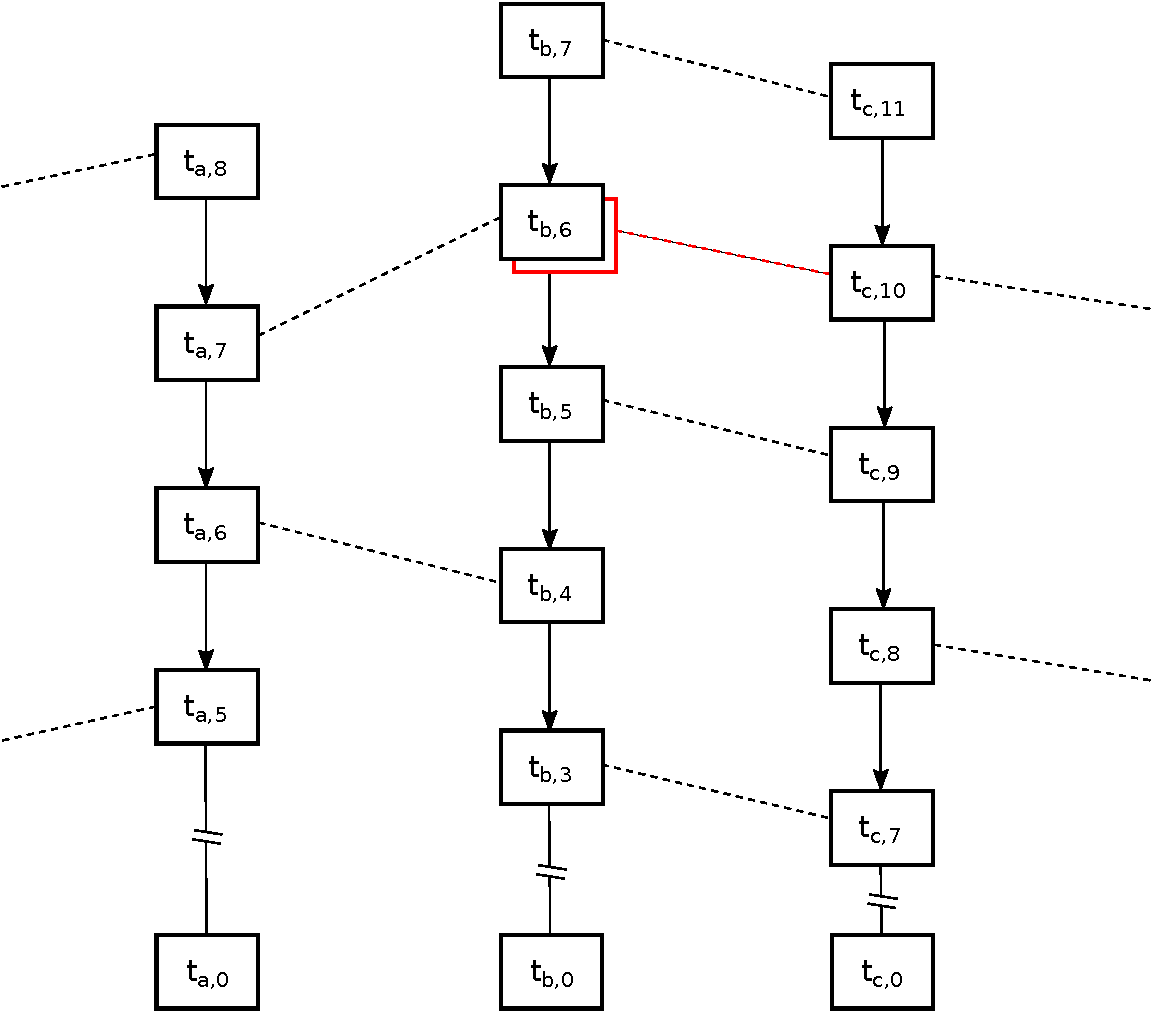
\includegraphics[width=0.9\textwidth]{trustchain-bad}
    \centering
    \caption{Every block is denoted by $t_{i,j}$, where $i$ is the node ID and $j$ is the sequence number of the block.
    Thus we have three nodes and three corresponding chains in this example.
    The arrows represent hash pointers and the dotted lines represent references.
    The blocks at the ends of one dotted line are pairs of each other.
    The red block after $t_{b, 5}$ indicate a fork.}
    \label{fig:trustchain-bad}
\end{figure}

If every node follows the rules of TrustChain and we only consider hash pointers,
then the chain effectively forms a singly linked list.
However, if a node violates the rules, then a \emph{fork} may happen.
That is, there may be more than one TX block with a hash pointer pointing back to the same block.
In \Cref{fig:trustchain-bad}, node $b$ (in the middle chain) created two TX blocks that both point to $t_{b, 5}$.
If this is a ledger system it can be seen as a double spend, where the currency accumulated up until $t_{b, 5}$ are spent twice.

\subsubsection*{Extended TrustChain}
We are now ready to explain the extended TrustChain, which we abbreviate to ETC.
In ETC, we introduce a new type of block, namely checkpoint (CP) block.
In contract to TX blocks, CP blocks do not store transactions or contain references.
They capture the state of the chain and the state of the whole system.
In particular, the state of the chain is captured with a hash pointer.
The state of the whole system is captured in the content of the CP block,
namely as a digest of the latest \emph{consensus result} which we explain in \Cref{sec:overview-cons}.
A visual representation is shown in \Cref{fig:trustchain-bad-cp}.

\begin{figure}
    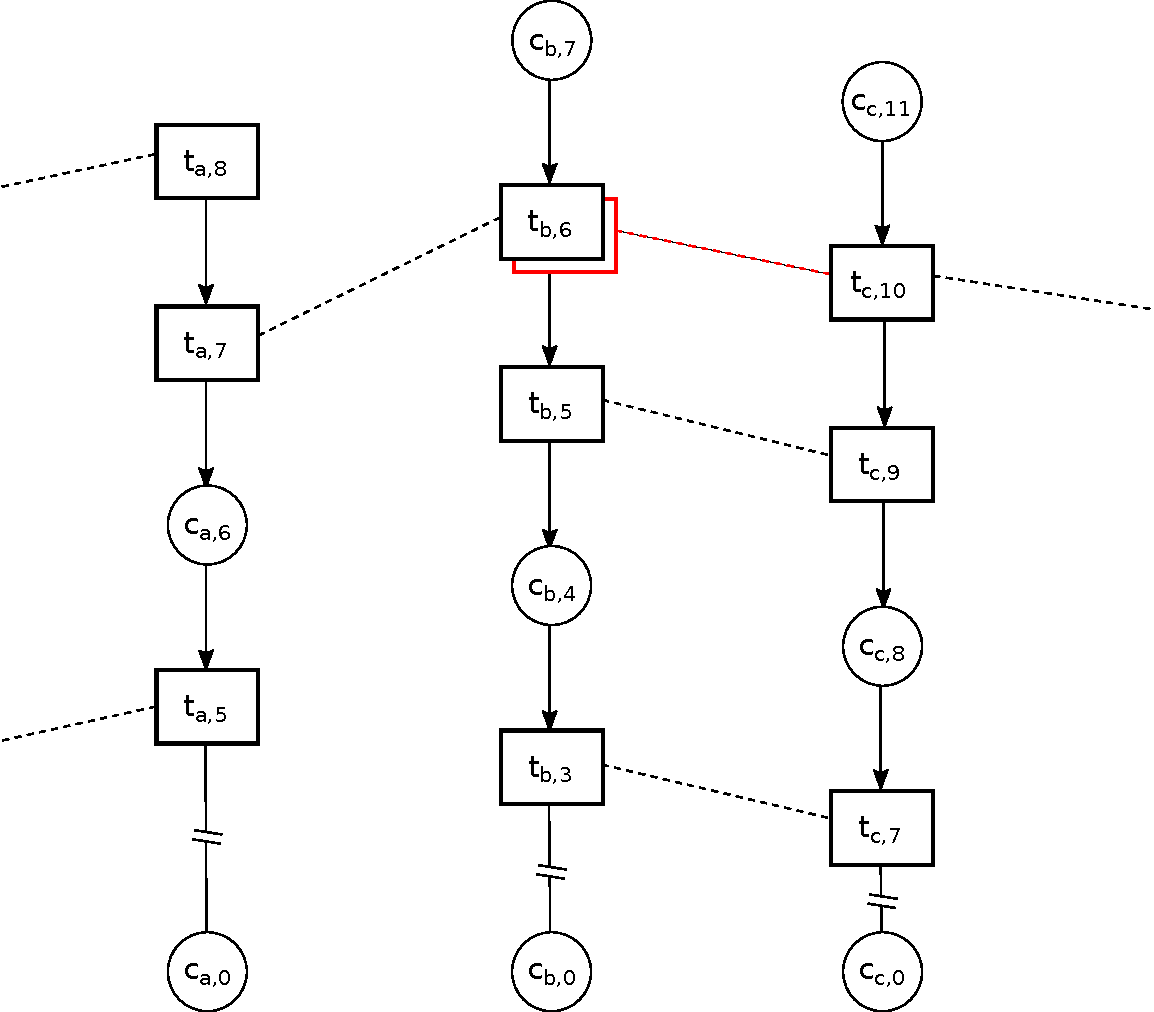
\includegraphics[width=0.9\textwidth]{trustchain-bad-cp}
    \centering
    \caption{The circles represent CP blocks,
    they also have hash pointers (arrow) but do not have references (dotted line).
    Note that the sequence number counter do not change, it is shared with TX blocks.}
    \label{fig:trustchain-bad-cp}
\end{figure}

\subsection{Consensus Protocol}\label{sec:overview-cons}
Before describing our consensus protocol, we take a brief detour to explain Byzantine consensus,
which is a fundamental building block of our consensus protocol.

\subsubsection*{Byzantine consensus}
Byzantine consensus is also known as \emph{atomic broadcast}.
Roughly speaking, atomic broadcast need to satisfy the following properties.
\begin{enumerate}
\item TODO
\end{enumerate}
TODO downsides (can't run with too many nodes) (high message complexity)
We stress that Byzantine consensus is not the same as Byzantine agreement or the Byzantine general's problem.
Byzantine agreement is TODO

The literature on Byzantine consensus and atomic broadcast is rich, some noteable ones include TODO.
Thus in the ETC consensus protocol, we assume there exist an "off-the-shelf" Byzantine consensus algorithm which we can use
(in our implementation we use HoneyBadgerBFT and motivate our choice in TODO).

In our case, every node do not propose some arbitrary data, but a set of CP blocks.
Thus the result of the consensus is the set union of all the legitimate proposals.

\subsubsection*{ETC consensus protocol} 
The consensus protocol runs continuously in rounds.
That is because a blockchain systems always need to reach consensus on new values, or CP blocks in our case.
This can be seen as running infinitly many rounds of some Byzantine consensus algorithm,
starting a new execution immediately after the previous one is completed.

As we mentioned earlier, the high message complexity prohibits us from running a Byzantine consensus algorithm on a large network.
Thus, for every round, we randomly select some node---called facilitators---to collect CP blocks,
and then use them as the proposal of the Byzantine consensus algorithm.
The facilitators are elected using a \emph{luck value}, which is computed using $H(\Cons_r || pk_i)$,
where $\Cons_r$ is the consensus result in round $r$ and $pk_i$ is the public key of $i$.
Intuitively, the election is guaranteed to be random 
because the output of a cryptographically secure hash function is unpredictable and $\Cons_r$ cannot be determined in advance.

A visual explaination can be found in \Cref{app:consensus-example},
it walks through the steps needed for a node to be selected as a facilitator.

\subsection{Transaction Protocol}
The TX protocol~\footnote{It is also known as True Halves, devised and implemented by Ewout Bongers.
See \url{https://github.com/Tribler/tribler/pull/2135} for more information.}
consist of two messages, \texttt{TX\_REQ} and \texttt{TX\_RESP}.
When a node  wishes to create a transaction,
it generates a TX block with the corresponding hash pointer, sequence number, counterparty and the transaction message itself.
It then sends a \texttt{TX\_REQ} message containing the TX block to the counterparty.
Upon receiving a TX block at the counterparty, it creates its own version of the TX block (the pair of the sender's TX block),
and sends it back to the sender in a \texttt{TX\_RESP} message.
At the end of the protocol, both parties should have both versions of the TX block.

\subsection{Validation Protocol}
The consensus and transaction protocol by themselves do not provide a mechanism to detect forks or other forms of tamperaing.
This is the goal of the validation protocol.

It also has two message---\texttt{VD\_REQ} and \texttt{VD\_RESP}.
When a node wishes to validate a transaction,
it sends a \texttt{VD\_REQ} with the sequence number $s$ to the party that created the TX block of the transaction.
Upon receiving a \text{VD\_REQ}, the node finds two \emph{agreed} CP blocks that surrounds the TX block and computes the \emph{fragment}.
An agreed CP block means that it has reached consensus.
A fragment of two CP blocks is a section of the chain where the beginning and the end are defined by those two CP blocks.
With the fragment, the node replies with a \texttt{VD\_RESP} message.
Upon receiving a \texttt{VD\_RESP}, the node checks that the fragment is created correctly.
Loosely, that means the agreed CP blocks have actually reached consensus,
the fragment has the correct hash pointers,
and TX block containing $s$ exists and is valid.


\subsection{Putting The Protocols Together}
The final protocol ($\Preal$) is essentially the concurrent composition of the three aforementioned protocols.
Our subprotocol design gives us the highly desireable non-blocking property.
In particular, we do not need to ``freeze'' the state of the chain for some communication to complete in order to create a block.
For instance, a node may start the consensus protocol, and while it is running, the node may still perform transactions.
By the time the consensus protocol is done, the new CP block is added to whatever the state that the chain is in.
It is not necessary to keep the chain immutable while the consensus protocol is running.


\section{Extended TrustChain Protocol}

\section{Protocol Extensions}

